\documentclass{sprawozdanie-agh}

\usepackage[utf8]{inputenc}
\usepackage{listings}
\usepackage{tikz}
\usepackage{xcolor}
\usepackage{graphicx}
\usepackage{caption}
\usepackage{lipsum}
\usepackage{wrapfig}
\usepackage{subcaption}
\usepackage{accsupp}
\usepackage{array}
\usepackage{multirow}
\usepackage{amsmath}
\usepackage{siunitx}    
\usepackage{pgfplots}
\usepackage{pgfplotstable}

\graphicspath{ {./images/} }
\pgfplotsset{compat = newest}

\usetikzlibrary{angles,quotes}
\makeatletter

\begin{document}

\przedmiot{Teoria Współbieżności}
\tytul{Laboratorium 8}
\podtytul{Petri Nets}
\kierunek{Informatyka}
\autor{Kyrylo Iakymenko}
\data{Kraków, 13 grudnia 2024}

\stronatytulowa{}

\section{Zadanie 1}

\begin{figure}[h!]
	\centering{
		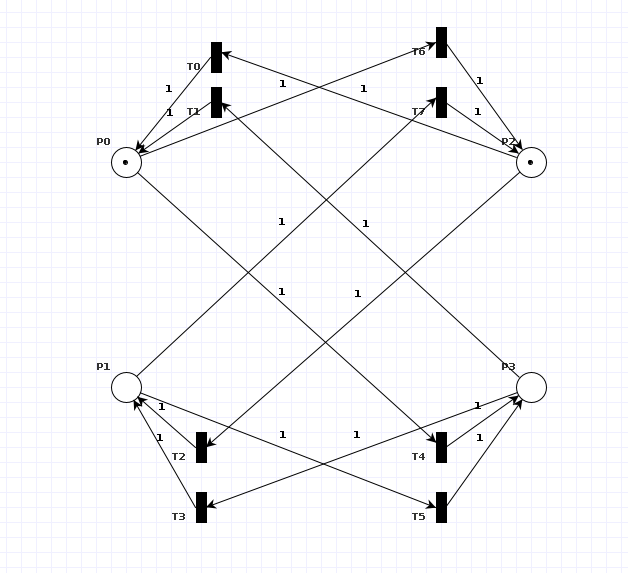
\includegraphics[width=0.67\textwidth]{img/bipartite.png}
	}
	\caption{Maszyna stanów}
	\label{zad2:graph1}
\end{figure}

\begin{figure}[h!]
	\centering{
		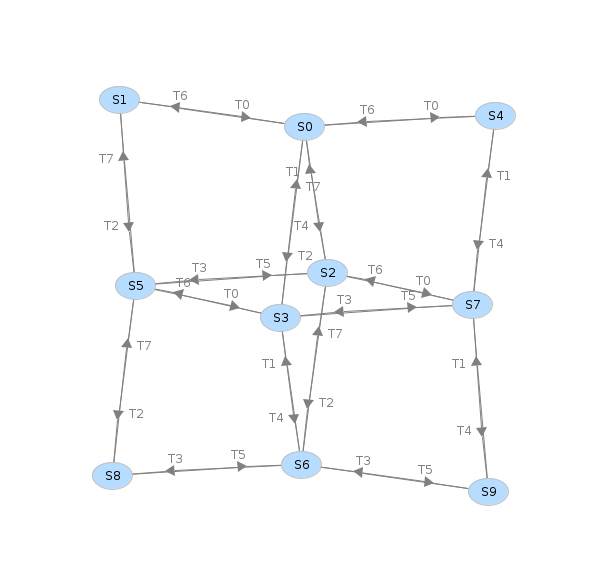
\includegraphics[width=0.67\textwidth]{img/bipartiteg.png}
	}
	\caption{Graf osiągalności maszyny stanów}
	\label{zad2:graph1}
\end{figure}

\subsection{Analiza grafu osiągalności}
\begin{itemize}
	\item Jak widać na grafie osiągalności - wszystkie stany są osiągalne.
	\item Sieć jest zachowawcza i $2$ - ograniczona, ale nie jest bezpieczna.
	\item Każde przejście jest krawędzią w grafie.
	\item Sieć jest żywa.
\end{itemize}


\subsection{Analiza niezmienników}
\quad Wiemy, że wszystkie możliwe rozkłady dwóch zasobów sieci są osiągalne. 
Więc jedynym niezmiennikiem miejsc jest $P_0 + P_1 + P_2 + P_3 = 2$, mówiący nam o tym, że 
sieć jest zachowawcza.

Podobna sytuacja z niezmiennikami przejść. Możemy wrócić do stanu początkowego przez 
dowolną krawędź w dwóch krokach.

\section{Zadanie 2}

\begin{figure}[h!]
	\centering{
		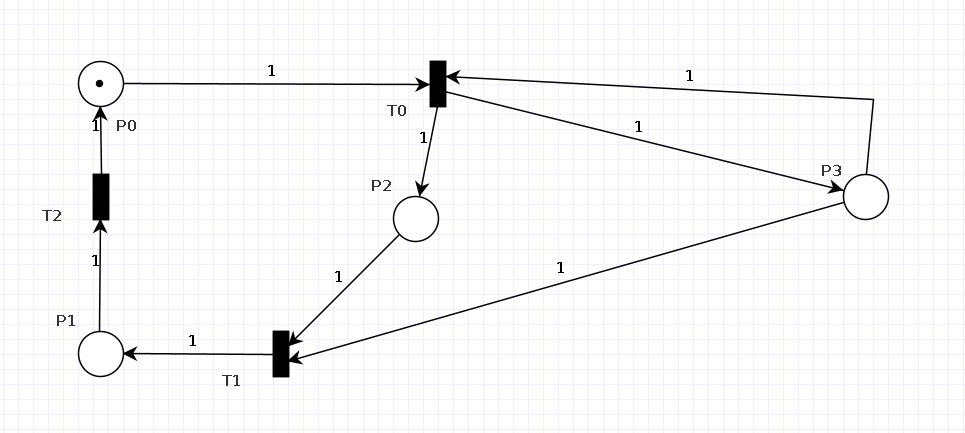
\includegraphics[width=0.67\textwidth]{img/21.png}
	}
	\caption{Sieć z podanego przykładu}
	\label{zad2:graph1}
\end{figure}

\begin{figure}[h!]
	\centering{
		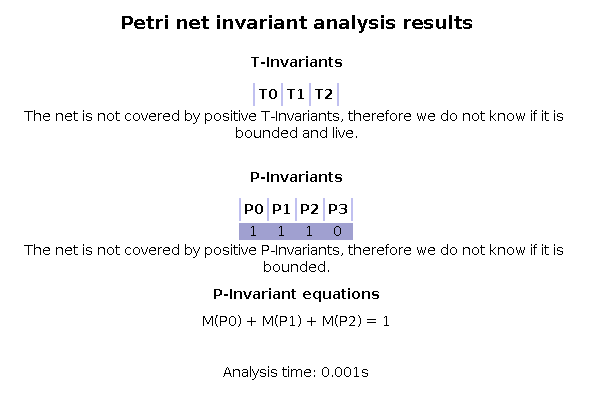
\includegraphics[width=0.67\textwidth]{img/23.png}
	}
	\caption{Niezmienniki sieci z podanego przykładu}
	\label{zad2:graph1}
\end{figure}
\begin{figure}[h!]
	\centering{
		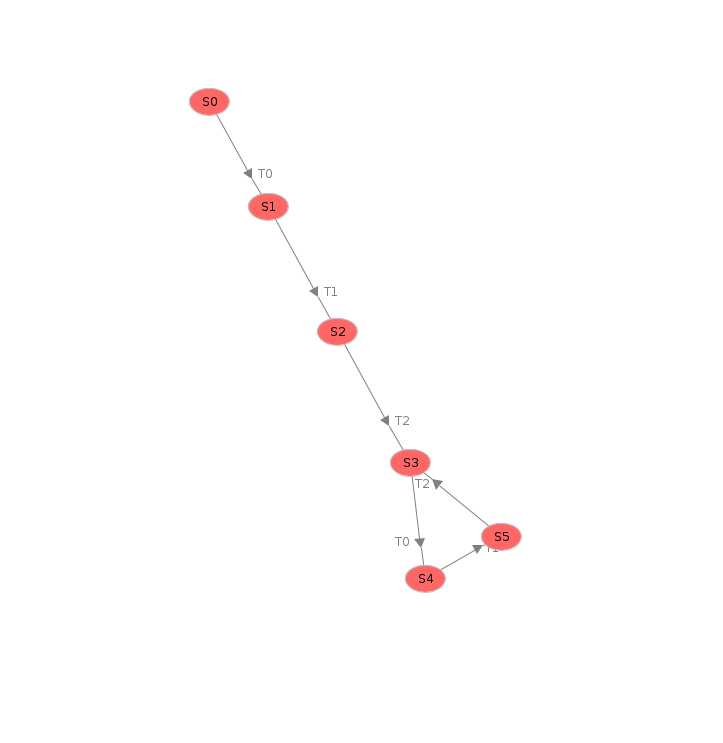
\includegraphics[width=0.67\textwidth]{img/2_3.png}
	}
	\caption{Graf osiągalności}
	\label{zad2:graph1}
\end{figure}
\newpage
\subsection{Graf osiągalności}
W miejscu $P_3$ może wystąpić dowolnie duża liczba, więc graf osiągalności jest nieskończony.
\subsection{Analiza niezminników przejść}
Sieć nie jest odwracalna, ponieważ możemy dodać dowolną ilość tokenów w 
stanie $P_3$.

\section{Zadanie 3}

\begin{figure}[h!]
	\centering{
		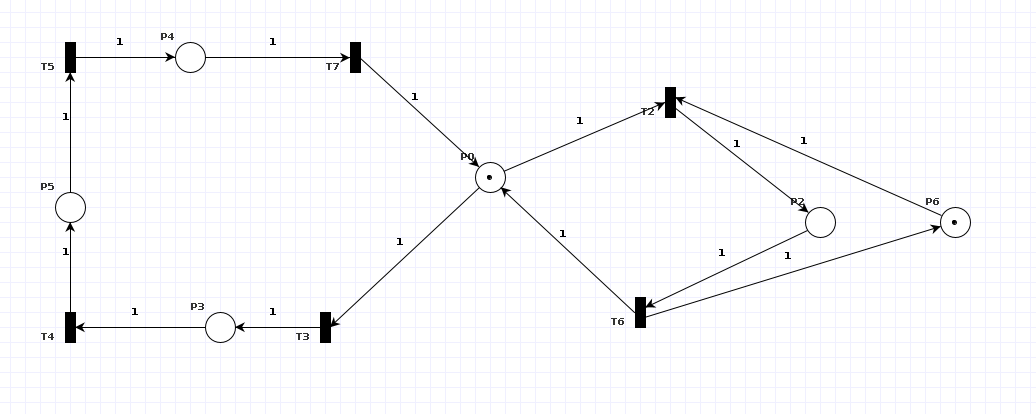
\includegraphics[width=0.67\textwidth]{img/2.png}
	}
	\caption{Sieć reprezentująca wzajemne używanie zasobów}
	\label{zad2:graph1}
\end{figure}
\begin{figure}[h!]
	\centering{
		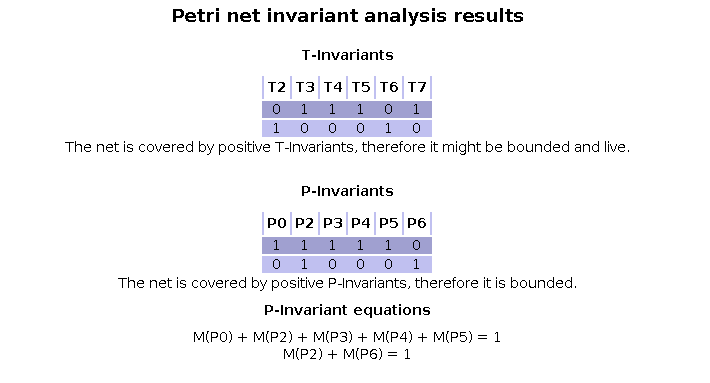
\includegraphics[width=0.75\textwidth]{img/kryt.png}
	}
	\caption{Niezmienniki sieci}
	\label{zad2:graph1}
\end{figure}

\subsection{Analiza niezminników sieci}
Równanie pierwsze chroni nam sekcję krytyczną. 

Równanie drugie wskazuje na to, że w każdym momencie dokładnie jeden z procesów 
po prawej stronie sieci jest uruchomiony.


\section{Zadanie 4}
\begin{figure}[h!]
	\centering{
		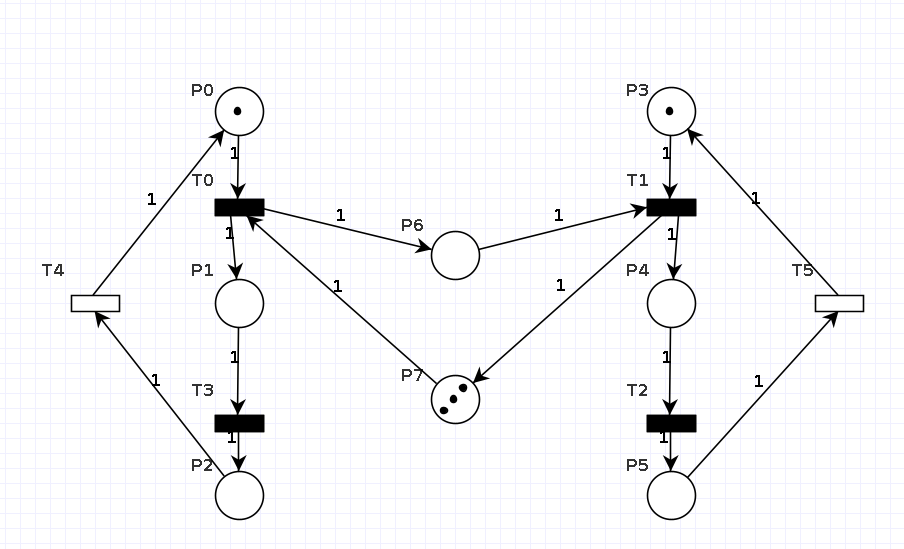
\includegraphics[width=0.67\textwidth]{img/buf.png}
	}
	\caption{Sieć reprezentująca bufor ograniczony}
	\label{zad2:graph1}
\end{figure}

\begin{figure}[h!]
	\centering{
		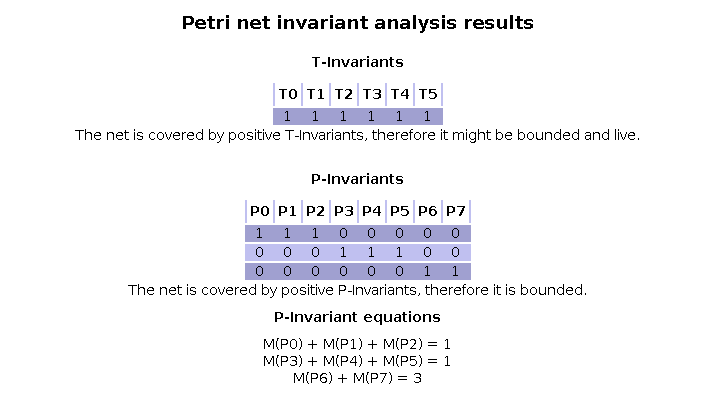
\includegraphics[width=0.67\textwidth]{img/2_1.png}
	}
	\caption{Niezminniki sieci}
	\label{zad2:graph1}
\end{figure}


\subsection{Analiza niezmienników}
Tak, sieć jest zachowawcza. 
Za pojemność bufora odpowiada ostatnie równanie.
\section{Zadanie 5}
\begin{figure}[h!]
	\centering{
		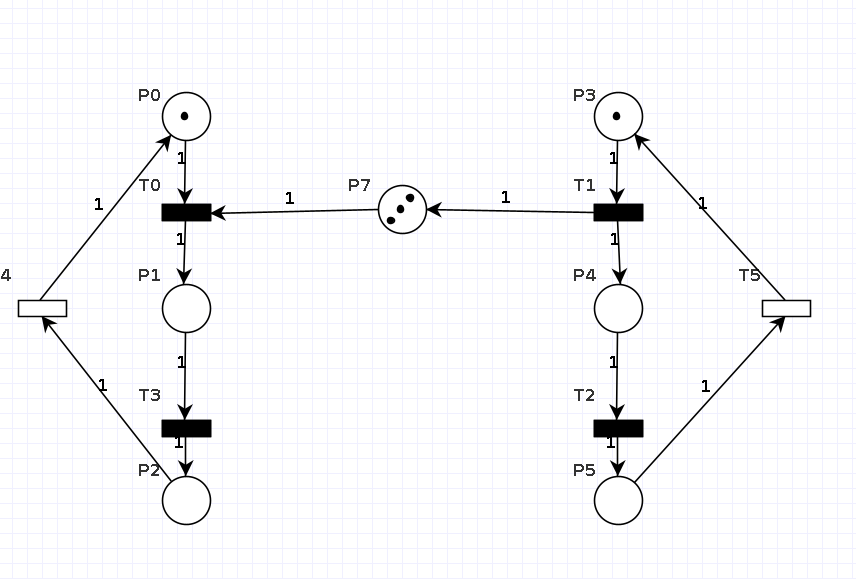
\includegraphics[width=0.67\textwidth]{img/buf2.png}
	}
	\caption{Sieć reprezentująca bufor nieograniczony}
	\label{zad2:graph1}
\end{figure}

\begin{figure}[h!]
	\centering{
		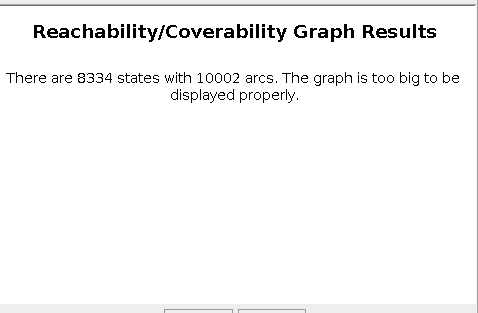
\includegraphics[width=0.67\textwidth]{img/buf2r.png}
	}
	\caption{Niezminniki sieci}
	\label{zad2:graph1}
\end{figure}

\subsection{Analiza niezmienników}
Można łatwo zaobserwować, że ze względu na bufor ($P_2$) sieć nie będzie ograniczona 
ani tym bardziej bezpieczna. 
Nie będzie także zachowawcza.

\subsection{Graf osiągalności}
Jak widzimy graf osiągalności jest za duży, żeby program go narysował. 
Czego warto było się spodziewać, gdyż sieć nie jest ograniczona.
\section{Zadanie 6}
\begin{figure}[h!]
	\centering{
		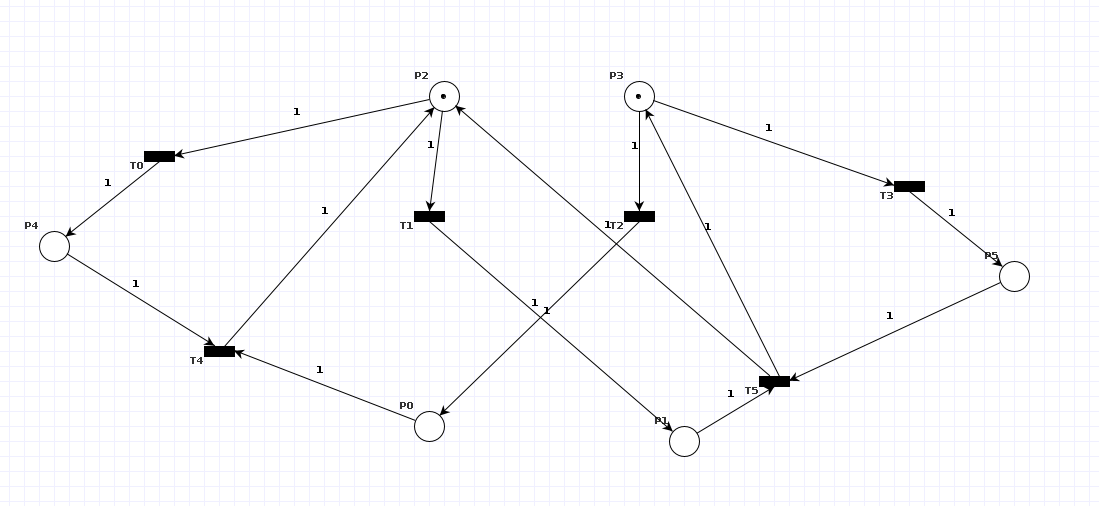
\includegraphics[width=0.67\textwidth]{img/d.png}
	}
	\caption{Sieć z deadlockiem}
	\label{zad2:graph1}
\end{figure}

\begin{figure}[h!]
	\centering{
		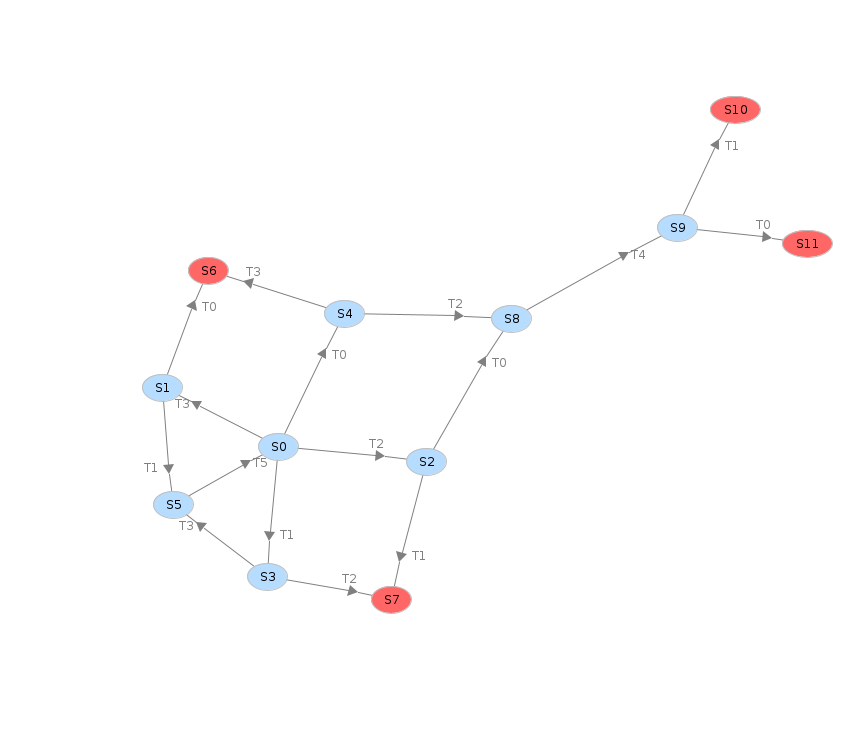
\includegraphics[width=0.67\textwidth]{img/dr.png}
	}
	\caption{Graf osiągalności}
	\label{zad2:graph1}
\end{figure}
\begin{figure}[h!]
	\centering{
		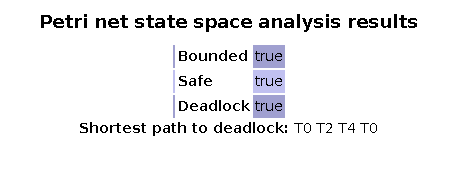
\includegraphics[width=0.67\textwidth]{img/dd.png}
	}
	\caption{Niezminniki sieci}
	\label{zad2:graph1}
\end{figure}

\subsection{Graf osiągalności}
Jak widzimy graf osiągalności posiada sekcje z których nie da się wyjść 
(zaznaczone na czerowno). Gdy sieć wchodzi do tego stanu następuje zakleszczenie.

\subsection{Analiza przestrzeni stanów}
Obecność zakleszczenia możemy także zaobserwować w tabeli analizującej 
przestrzeń stanów naszej sieci.
% \begin{thebibliography}{3}

% \bibitem{teams_materials}
% Materiały pomocnicze do laboratorium zamieszczone na platformie Teams w~katalogu \emph{lab01/lab1-intro.pdf}.


% \bibitem{underflow_wiki}
% Artykuł o `Arithmetic underflow` z wikipedii \url{https://en.wikipedia.org/wiki/Arithmetic_underflow}.

% \end{thebibliography}

\end{document}
